% Chapter Template

\chapter{Correct by Construction Agile Scrum Technique} % Main chapter title

\label{Chapter_Applying_the_methodology} % Change X to a consecutive number; for referencing this chapter elsewhere, use \ref{ChapterX}

We have now described the process we are going to follow. In this chapter, we describe 
the technique we are going to use the create the artefacts.

To create all the artefacts we need a mathematical specification language and a 
programming language.

\section{Mathematical Specification Language (TLA\textsuperscript{+})}

The Formal Specification and Formal Design has to be written in a formal
mathematical language. CbyC suggests using Z  \parencite{CbyCPraxis}. 
I hound that Z has very little tool support and an inactive community. I decided
to use TLA\textsuperscript{+}.  TLA\textsuperscript{+} has frequently updated 
tooling and an active community. To get started with TLA\textsuperscript{+}
visit the ``Learning TLA\textsuperscript{+}'' website \parencite{LearningTLA}.

Using TLA\textsuperscript{+} we specify a system as a set of possible behaviours 
representing a correct execution of the system. We define a behaviour as a sequence
of states. A state is defined as an assignment of values to variables \parencite{SpecifyingSystems}.

\begin{figure}[H]
	\centering
	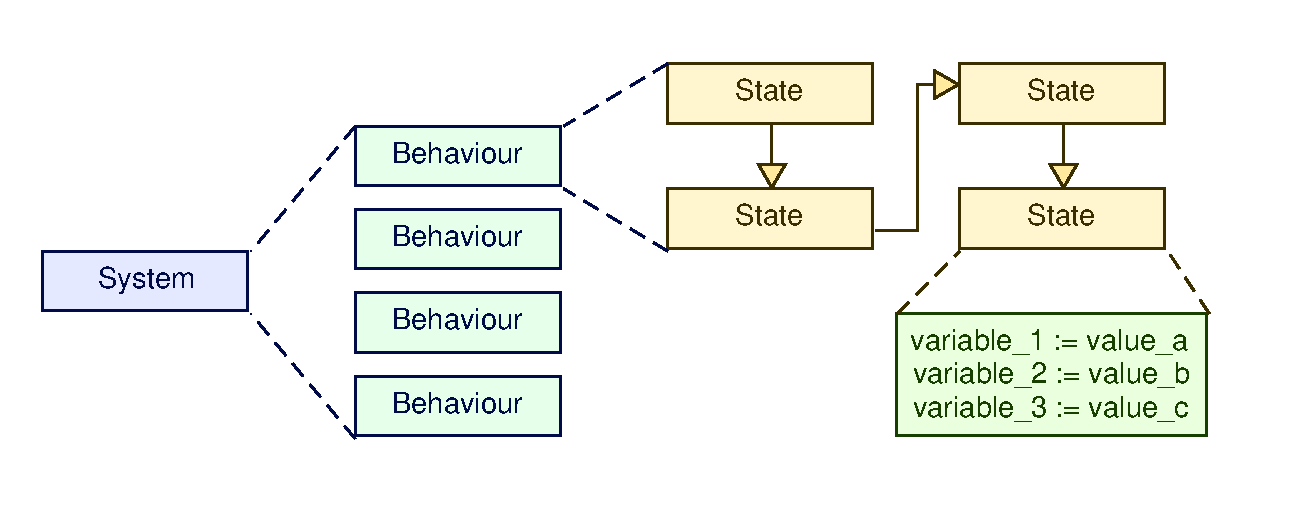
\includegraphics[scale=0.75]{Figures/System_Specification.pdf}
	\decoRule
	\caption{System specification.}
	\label{fig:SysSpec}
\end{figure}

\subsection{Writing a specification}

In listing \ref{code:AsynchInterfaceSpec} we show the complete TLA specification of the 
asynchronous data interface as described in appendix \ref{AppendixA}. The TLA\textsuperscript{+} Toolbox can generate a 
pretty version as shown in figure \ref{fig:PDFCode}

The specification formula, \( Init \land \Box\left[ Next \right]_{\langle value, ready, acknowledge \rangle} \),
states that the initial state \(Init\) must be true at the start and that all 
subsequent states must be states specified by \(Next\).

The valid behaviours are defined by the \(Next\) formula. It is split into \(Send\) and \(Receive\) states.

TLA\textsuperscript{+} is an untyped language. Type correctness is checked by creating an invariant, 
\(TypeInvariant\), defining valid values for each variable \parencite{SpecifyingSystems}.

\(EXTENDS \ Naturals\) imports the \(Naturals\) standard module. The \( Naturals\) module defines the set of natural
numbers and operator like \(+, -, \dots\) \parencite{ModelCheckingTLASpecifications}.

\(CONSTANTS\  Data\) declares that \(Data\) is a constant. We define the values in the 
\(Data\) set when setting up the model checker.

\( VARIABLES \ value, ready, acknowledge\) declares that \(value\), \(ready\), and \(acknowledge\) are variables.

\vspace{5mm} %5mm vertical space

\begin{lstlisting}[frame=single, language = TLA, literate={-}{{-\allowbreak}}{1}, caption={Asynchronous data interface specification.}, captionpos=b, label={code:AsynchInterfaceSpec}]
--------------- MODULE AsynchInterface ---------------
EXTENDS Naturals
CONSTANTS Data
VARIABLES value, ready, acknowledge
TypeInvariant == /\ value \in Data
                 /\ ready \in {0,1}
                 /\ acknowledge \in {0,1}             
------------------------------------------------------
Init == /\ value \in Data
        /\ ready \in {0,1}
        /\ acknowledge = ready
        
Send == /\ ready = acknowledge
        /\ value' \in Data
        /\ ready' = 1 - ready
        /\ UNCHANGED acknowledge
        
Receive == /\ ready /= acknowledge
           /\ acknowledge' = 1 - acknowledge
           /\ UNCHANGED <<value, ready>>
              
Next == Send \/ Receive
Spec == Init /\ [][Next]_<<value, ready, acknowledge>>
------------------------------------------------------
THEOREM Spec => []TypeInvariant
======================================================
\end{lstlisting}

\begin{figure}[H]
	\centering
	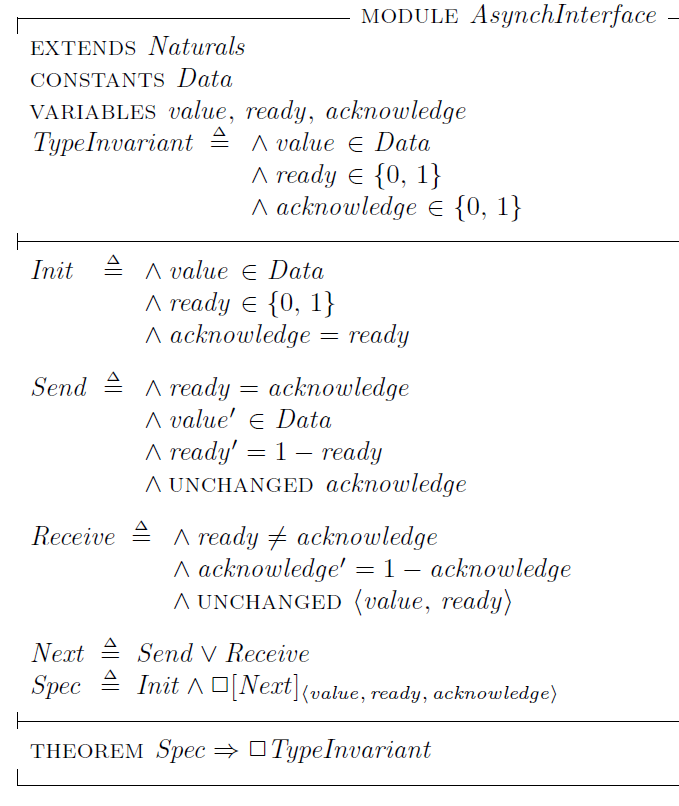
\includegraphics[scale=0.75]{AsynchInterface_Code.png}
	\decoRule
	\caption{PDF code.}
	\label{fig:PDFCode}
\end{figure}

\subsection{Evaluating a specification}
We evaluate a specification using the TLC model checker. The model checker is available as part of the 
TLA Toolbox \parencite{The_TLA_Toolbox}.

TLC explores reachable states, looking for a state in which an invariant is not satisfied or
deadlock occurs. Deadlock happens when there is no possible next state. TLC stops 
when it has examined all states reachable by traces that contain only states
satisfying the mode constraints \parencite{ModelCheckingTLASpecifications}.

\section{Programming Language (C\#)}

CbyC suggests using the Ada SPARK programming language because it has native
support for code contracts and can verify the code using static analysis \parencite{CbyCPraxis}.
Very little line-of-business software is built using Ada. To make this more relevant 
to the my work I decided to use C\#. The problem with C\# is that is has no native
support for code contracts and also does not have sufficient static analysis tools 
capable of verifying code correct. This means that we will have to find workarounds
for these short comings. 

\subsection{Code Contracts}

CbyC program design is based on information flow expressed as code contracts 
\parencite{CbyCMan}. C\# does not have native code contracts any more \parencite{NoCodeContracts},
but it is very simple to implement code contracts using standard C\# language features.

Code contracts are an application of Hoare logic. Using Hoare logic
we can show that a program correctly implements a specification if, given a set of 
preconditions derived from the specification, the program never violates a set of
post conditions derived from the specification. We use the Hoare triple to 
represent the contract \parencite{BasisForProgramming}:

\[
	\{P\}Q\{R\}
\]

where:
\begin{description}
	\item [\(P\)] are the preconditions;
	\item [\(Q\)] is the program;
	\item [\(R\)] are the postconditions.
\end{description}

With some helper methods we can implement code contracts using standard C\# language
features. We are modelling our code contracts on the Design by Contract design 
\parencite{ObjectOrientedSoftwareConstruction}.

Design by Contract has two specification levels:
\begin{itemize}
	\item method preconditions and postconditions;
	\item class invariants.
\end{itemize}

Preconditions are a set of conditions that state what the method requires from 
the client (code calling the method) in order to function correctly.

Postconditions are a set of conditions that state what the method will ensure 
happens at the end of it's execution.

Class invents are a set of conditions that will always be true after any 
execution. 

The action to be performed when a contract fails depends on what you want. There 
are two possible actions, either throw an exception causing the program to stop or
log a message that you can use for debugging.

\vspace{5mm} %5mm vertical space

\lstset{style=sharpc, captionpos=b, caption={Writing code contracts using helper methods.}}
\begin{lstlisting}[frame=single]
public class Account
{
    private int _limit;
    public int Limit
    {
        get => _limit;
        set
        {
            Require(value > 0, "Limit must not be 0.");
            _limit = value;
            ClassInvariant();
        }
    }

    public int Total { get; private set; }

    public int Add(int value, int discount)
    {
        Require(value >= 0, "Value must be positive.")
        .Require(
            discount >= 0 && discount <= 50, 
            "Discount must be positive and not more than 50%");
        var old = new { Total };

        // method logic

        Ensure(Total > old.Total, "The total will not decrease.");
        ClassInvariant();
        return discountedValue;
    }

    private void ClassInvariant()
    {
        Invariant(Total >= 0, "The total will not be negative.")
        .Invariant(Limit > 0, "Limit will not be 0.");
    }
}
\end{lstlisting}

\subsection{Verification}

Using unit testing to verify code correct is not always effective. The code contracts 
encode the specification, we there for only have to show that the code we wrote 
does not breach the contract to verify the code.

We can represent a program or section of a program, unit, as a mathematical function
(\(f\)). All possible legal permutations of inputs are the function's domain (\(I\)) and 
the outputs are the function's range (\(O\)).

\[ f: I \rightarrow O \]

It would be impractical to write unit tests that cover the complete domain
of a unit. Instead we randomly select inputs from the domain. When we tests smaller
units, random testing is adequate \parencite{Hamlet94randomtesting}.
We are not going to verify the outputs because,
if the outputs adhere to the contracts we assume the outputs are valid. This will 
eliminate the oracle problem \parencite{QuickCheck}\parencite{Hamlet94randomtesting}.

We will be using FsCheck to select the random inputs. FsCheck is a .net implementation
of QuickCheck \parencite{FsCheck_home}. We use the xUnit test framework to make
writing the test more convenient.

The tests have two parts, the input generators and tests action. We first look at the generators.
We group the test inputs using tuples. The generator code filters the generated value according
to the contracts.

\vspace{5mm} %5mm vertical space

\lstset{style=sharpc, captionpos=b, caption={FsCheck generators.}}
\begin{lstlisting}[frame=single]
public static class Arbitraries
{
    public static Arbitrary<(decimal limit, decimal total)> ...
        ... AccountGenerator()
    {
        return (
            from limit in Arb.Default.Decimal()
                            .Convert(
                                limit => limit.Round(), 
                                limit => limit)
                            .Filter(limit => limit > 0)
                            .Generator
            from total in Arb.Default.Decimal()
                            .Convert(
                                total => total.Round(), 
                                total => total)
                            .Filter(total => total > 0)
                            .Generator
            where total < limit
            select (limit, total))
        .ToArbitrary();
    }

    public static Arbitrary<(decimal value, decimal discount)> ...
        ... AccountAddGenerator()
    {
        return (
            from value in Arb.Default.Decimal()
                            .Convert(
                                value => value.Round(),
                                value => value)
                            .Filter(value => value >= 0)
                            .Generator
            from discount in Arb.Default.Decimal()
                            .Convert(
                                discount => discount.Round(), 
                                discount => discount)
                            .Filter(discount => 
                                discount >= 0 && discount <= 50)
                            .Generator
            select (value, discount))
        .ToArbitrary();
    }
}
\end{lstlisting}

 We then use the random inputs to set up a test account and then add a value.
We do not assert anything after the test because we just want to show that the contracts are not 
violated. 

\vspace{5mm} %5mm vertical space

\lstset{style=sharpc, captionpos=b, caption={FsCheck property.}}
\begin{lstlisting}[frame=single]
[Property(Arbitrary = new[] { typeof(Arbitraries) }, Verbose = true)]
public void AddProperty(
    (decimal limit, decimal total) accountSetup,
    (decimal value, decimal discount) accountAdd)
{
    // ARRANGE
    var account = new Account(accountSetup.total, accountSetup.limit);

    // ACT
    account.Add(accountAdd.value, accountAdd.discount);
}
\end{lstlisting}

\vspace{5mm} %5mm vertical space

\lstset{captionpos=b, caption={Generated FsCheck test data.}}
\begin{lstlisting}[frame=single]
0:
((0.73063M, 0.21486M), (0.92590M, 0.35410M))

1:
((0.59390M, 0.55137M), (0.72667M, 0.19132M))

...

98:
((20.83859M, 15.16400M), (42.22400M, 26.75752M))

99:
((48.77803M, 20.94168M), (29.58231M, 2.28041M))
\end{lstlisting}
